\section{Study with University Students}

As presented in Chapter \ref{cha:method}. It was proposed to students, as one of the activities 
of the Free Software course, that they make the first-time contribution to the Linux kernel to 
mitigate duplication found by the ArKanjo tool while sending patches to the Linux subsystem 
maintainers and documenting their experiences and learnings.

For the students who worked in the IIO subsystem, the teaching assistant gave them duplicated 
function pairs 
found by the tool, and their responsibility was to think of how to mitigate the duplication 
and send the patch to the maintainers. The student that worked in the AMD Display driver 
have the additional work to use the tool to find the duplications.

Appendix \ref{app:stuart} has references to the artifacts discussed in this section, 
including the duplication function pairs that students mitigate, the students’ reports, 
the patch students sent to the Linux kernel, and the answers to the survey asked 
of the student who worked in the AMD Display driver and the teaching assistant that used 
the tool to find duplications in the IIO subsystem.

\begin{table}
\begin{tabular}{ | c | c | c | c | m{6em} | }

\hline

\textbf{Group} & \textbf{Subsystem} & \textbf{Lines added} & \textbf{Lines removed} & \textbf{Refactoring methods used}
\\ \hline 

1 & IIO & 7 & 14 & None \\ \hline
2 & IIO & 23 & 24 & Parameterize method \\ \hline
3 & IIO & 12 & 30 & Parameterize method \\ \hline
4 & IIO & 2 & 7 & None \\ \hline
5 & IIO & 17 & 70 & Parameterize method \\ \hline
6 & IIO & - & - & Parameterize method \\ \hline
7 & IIO & 21 & 22  & None \\ \hline
8 & IIO & - & - & None \\ \hline
9 & IIO & 33 & 52 & Parameterize method \\ \hline
10 & IIO & 32 & 58 & Parameterize method \\ \hline
11 & IIO & - & - & Parameterize method \\ \hline
12 & AMD & 89 & 489 & None \\ \hline

\hline
\end{tabular}
\caption{Refactor methods used and metrics of the students's mitigations.}
\label{tab:stu}
\end{table}


Table \ref{tab:stu} summarizes students' groups' mitigation approaches. Seven groups applied 
the parameterized refactor method, 
and two applied the extractor method to their approaches to mitigate the duplications. 
The other three groups do not use any refactor methods presented in the literature.  
Five groups got their patches accepted and merged in Linux; four groups got their patches rejected, 
and one group is still working on the patch submission, being in the fifth version of the patch at 
the time this document was written. Two groups decided not to continue sending the patches after 
they made initial versions.

Groups one and four have worked in similar duplications, where two functions return a 
boolean mirroring the results. That means when the first function returns true, the second 
function returns false, and when the first function returns false, the second function 
returns false. Group one had a simple approach, and the maintainers approved the changes quickly. 
Group four attempted to mitigate the duplication with macros, a method found in the code file 
they were working on. The maintainers disagreed with the proposed approach, arguing that the 
proposed changes decrease the code readability, and asked for an approach similar to group one. 
Group four submitted the patch after coding the approach proposed by the maintainers.

Groups three, six, and ten created a struct to encapsulate the parameters and mitigate duplication 
when applying the parameterized method. Group three sent the mitigation to the maintainers and 
approved it without significant comments. In contrast, the patch from group ten was rejected by 
the same maintainer who approved the patch from group three. The maintainer justification to reject 
the patch is that group ten refactored code files that has simple context, therefore adding a layer 
of abstraction to remove a duplication deacrease the code readability without clear gains on 
the codebase quality. Figure \ref{fig:group_10_reply} shows the maintainers's feedback for group ten.


\begin{figure}
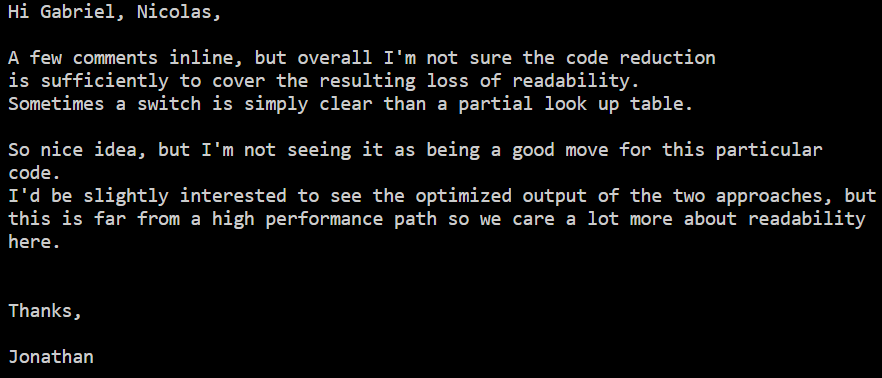
\includegraphics[scale=0.8]{group_10_reply}
\caption[Maintainers' Feedback on Group Ten's Patch]{
Maintainers' Feedback on Group Ten's Patch
\footnote{Image obtained from Linux Lore, which is publicly provided at:
\url{https://lore.kernel.org/linux-iio/20250428034222.318898-1-gabrielgeraldinosouza@gmail.com/T/\#u}}
}
\label{fig:group_10_reply}
\end{figure}

Groups seven and eight used the extract method to approach the mitigations. Group eight sent the 
mitigations to the maintainers, and the code changes were approved, with minor requested changes 
in code style and smaller errors fixed. For group seven mitigation, the maintainers reject their 
patch because the code changes add layers of abstractions to the code, making it more complex and 
challenging to read. The maintainers proposed that group seven remove the duplicated functions and 
insert the duplicated code multiple times where the functions were being called. This suggestion 
may be bad practice for code quality, as it adds more complexity and responsibility to a bigger 
function; it is viewed as the best choice for removing layers of abstraction and making the 
code easier to read. Figure \ref{fig:group_7_reply} shows the maintainers's feedback for group seven.


\begin{figure}
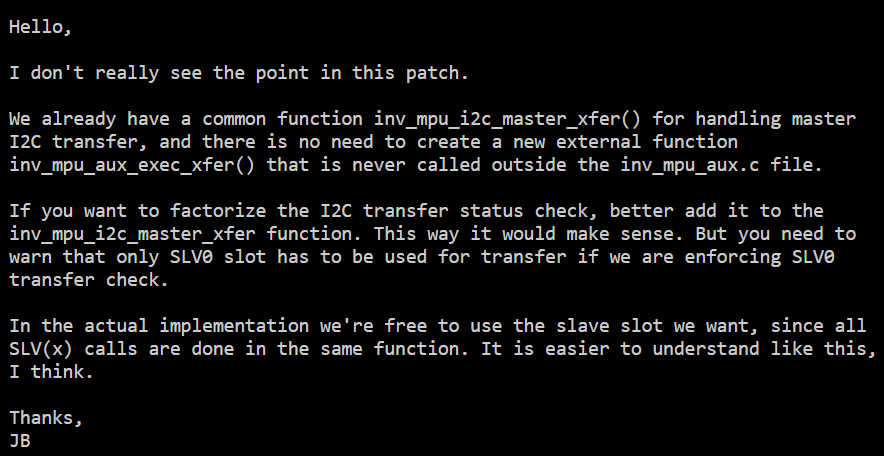
\includegraphics[scale=0.8]{group_7_reply}
\caption[Maintainers' Feedback on Group Seven's Patch]{
Maintainers' Feedback on Group Seven's Patch
\footnote{Image obtained from Linux Lore, which is publicly provided at:
\url{https://lore.kernel.org/linux-iio/20250428132551.176788-1-bellacaselli20@gmail.com/}}
}
\label{fig:group_7_reply}
\end{figure}

Groups nine and eleven faced similar issues to those in Mitigation 1 on our participant observation 
experiment, where configuration files designed as macros complicated the approach to the mitigations. 
Group nine applied the parameterized method to not need to know the configurations in the 
generic function, which is reasonable as the duplication approach only depends on one configuration 
value. Group eleven worked with multiple configuration values, and to refactor the duplication, 
they proposed to create a bigger macro that encapsulates the other macros, which is a clever 
solution but adds abstraction and complexity to macros, which makes the code harder to debug and read.
We do not get the feedback of the maintainers on the group eleven approach to know their opinions.

Group twelve is the student who executed the tool and passed through the process of finding 
duplications. The student found a duplication in the driver that happened across eighteen code files, 
creating a patch to remove four hundred lines of duplicated code. The student sent the mitigations 
to the maintainers, and their feedback pointed to fixing the warning in the code without arguing 
about removing the duplications.

Analyzing the students' approaches to the duplications and the maintainers' feedback, we saw that 
people without previous experience in Linux kernel development could approach duplications found 
by the ArKanjo tool and become contributors to the kernel. We observed that not all duplications 
are viewed as code with bad quality, with the maintainers analyzing the trade-off between the 
purpose of the duplicated code, code readability, and the levels of abstraction added to 
address the duplications.

\subsection{Survey Results Analysis}

We asked the teaching assistant and the students who used the ArKanjo to answer a survey with 
some questions related to the tool experience, such as installation, documentation, facility of 
use, new ideas to improve the tool, etc. Appendix \ref{app:survey} has the complete survey 
with the answers.

Related to the tool installation, neither the teaching assistant nor the students faced issues 
installing on the Debian distributions. However, the teaching assistant attempted to install it 
in the Arch Linux distribution and failed to install it on this Linux distribution. 
Regarding the tool's documentation, the teaching assistant pointed out errors that worsened his 
experience. The student asked for more examples and tutorials on using the tool in text or 
video formats.

On the ArKanjo tool preprocessing step, the student reported problems of disk space usage and 
crash errors, which we knew could happen as the tool iterates and can save information about 
every pair of functions in a codebase, as we did not implement any mechanism to control the 
memory usage. The teaching assistant reported only being able to execute the preprocessor with 
the text similarity method, and the diff method kept running for hours without finishing. 
The teaching assistant's report was unexpected behavior for us, as the text similarity method 
initially looked more complex; in contrast, the \textit{diff} method is a simple counter of equal lines 
with an operation system default command. The teaching assistant report corroborates the 
gensim efficiency \citep{gensim}.

Related to the tool's functionalities, both the student assistant and the student reported 
a missing mechanism to save the tool results on a separate file instead of the terminal output. 
The tool, by default, outputted with colors, as shown in section \ref{subsec:func}, which complicates 
redirecting the terminal output to a file.

We asked for the overall impression of the tool and if it met their expectations. We also asked 
them to give a score of one to five for installation, documentation, preprocessing, and functionalities. 
Both the teaching assistant and the student scored at least four on each mentioned point, thought that 
the tool fulfilled their expectations, and had an overall good experience. Finally, the teaching assistant 
the the student reported features ideas to the tool that may be interesting, which 
are showed below.

\paragraph{List of Possible Improvements}

\begin{itemize}

\item Enable the possibility of having several codebases of preprocessor artifacts and selecting one of them.

\item Add different methods to find duplication.

\item Adding more filters to search for duplicates, such as finding duplicates with more than 90\% 
similarity and more than 20 lines repeated.

\item Add options to highlight and filter duplications on the same file or directory.

\item Addition of support to save the tool output in files without manual preprocessing of the colored output.

\end{itemize}

With the survey feedback, we understood that users had a good experience and found value in the 
ArKanjo tool. They also provided critical points that could be improved. The most critical 
reported issues, such as documentation errors and a lack of support for multiple Linux distributions 
and different operating systems, have been fixed. Less critical issues remain open points that 
can be addressed in future work.

\subsection{Students Contribution to the Tool}

We listed multiple issues in the tool for the two groups that opted to contribute directly 
to developing the ArKanjo tool. The first group opted to work on expanding the tool's support 
for multiple operating systems. Some libraries used in the tool development only supported the 
Ubuntu distribution, and the first group was responsible for migrating these libraries to 
libraries with support for multiple operating systems. This issue was of our knowledge and 
was pointed out by the teaching assistant in the survey, as he reported the problem while 
using the tool.

The second group opted to work on a webpage for the tool documentation and support for 
light and dark modes. The colored output presented in the figures in Chapter \ref{cha:tool} was 
hard coded at first, not considering the user terminal colors, thus giving a bad user experience. 
The website helps facilitate people's contribution or use of the tool. We did not know how to 
approach the light and dark modes at first and did not need to look at how to fix the issue as 
the group searched and found a solution.

The students successfully delivered the issues proposed. We found it interesting to see 
people able to contribute to the tool on the problems that we did not even know how to approach.
The issues help the user experience and facilitate other research using the ArKanjo tool that 
we may explore in future works. Appendix \ref{app:contribution} references the 
students' contributions, the issue list proposed to the students, and figures from 
the documentation webpage.
